
\chapter{DiscordBotを作ってみよう}
\section{はじめに}
はじめまして、sudaです。私はDiscordで人とチャットをしている時に同じ会話が頻繁に続き、これBotで返事をするようにしたら返事をする手間が省けるし面白いのでは?と思いBotを作ることにしました。
発想がひどいって!?まあでも自分の発想したものを形にすることが面白いことだと思うので今回はそこには目を瞑りましょう…
もちろん自分が送ったメッセージに対してBotに返答させることもできるので、自分だけのオリジナルDiscordBotを作ってみましょう!

\section{何を作るのか}
Discordのサーバで特定のメッセージが来たら、特定のメッセージを返すDiscordのBotを作ります。
サンプルプログラムを参照したい方は以下のURLからご覧下さい。
\footnote{今回作るDiscordBotのサンプルプログラム\url{https://github.com/sudamichiyo/Discord_Bot_sampleprogram}}
例えば自分が「仕事終わった」と言うとBotが「お疲れ様」と返してくれます。
\section{実行環境・使用技術}
\begin{itemize}
  \item Python 3.10.8
\end{itemize}


\section{ローカル環境でBotが動作するようにする}
まずはローカル環境でBotが動作するようにしてみます。

\subsection{Botの作成・管理をする}
初めに、機能などはまだついていないBotをDiscordのポータルサイトから作成します。
DiscordのBotの作り方(メモ)という記事の「1.Discord上のBotの作成」を見ながらBotを作成してみて下さい。
\footnote{DiscordのBotの作り方(メモ)\url{https://note.com/exteoi/n/nf1c37cb26c41 (参照2023.3.29)}}

\subsection{ファイルの作成}
Botを実行するPythonファイルを作ります。
\begin{shaded}
  \begin{verbatim}
$ mkdir message_discord_bot
$ cd message_discord_bot
$ touch main.py
\end{verbatim}
\end{shaded}

\subsection{discord.pyの準備}
ここからはライブラリ(discord.py) のドキュメントを見ながら環境構築をしていきます。
\footnote{discord.pyドキュメント\url{https://discordpy.readthedocs.io/ja/latest/intro.html\#basic-concepts (参照2023.3.29)}}
PythonでDiscordのAPIを操作するために必要なライブラリをインストールします。先ほど作成したディレクトリにアクセスして、以下のコマンドで discord.py をインストールします。
\begin{shaded}
  \begin{verbatim}
$ python3 -m pip install -U discord.py
\end{verbatim}
\end{shaded}
次に、先ほど作成したmain.pyを以下のソースコードに書き換えます。
\begin{tcolorbox}[breakable]
  \begin{verbatim}
1 import discord
2 
3 class MyClient(discord.Client):
4     async def on_ready(self):
5         print(f'Logged on as {self.user}!')
6 
7     async def on_message(self, message):
8         print(f'Message from {message.author}
9                                         : {message.content}')
10
11 intents = discord.Intents.default()
12 intents.message_content = True
13
14 client = MyClient(intents=intents)
15 client.run('my token goes here')
\end{verbatim}
\end{tcolorbox}
ここで、以下のボットに関する2つの設定をDiscordのポータルサイトから設定してください。
\begin{itemize}
  \item ポータルサイトの「Bot」からトークンを取得する
  \item ポータルサイトの「Bot」の「MESSAGE CONTENT INTENT」を有効にする
\end{itemize}
'my token goes here'は取得したBotのアクセストークンを書きます。
以上の設定が終わったところで python3 main.py を実行すると、Botのサーバが立ち上がります。Bot のいるサーバの任意のチャンネルでメッセージを投稿すると
、コマンドライン上に「書いた人」と「メッセージ」がそのまま出力されます。

\subsection{環境変数の設定}
ソースコードに直接トークンを書いてしまうと、Githubでソースコードをホスティングするときにトークンキーが他の人にバレてしまいます。
これを防ぐために.envファイルを作成して、その中にDiscordのアクセストークンを書きます(下記参照)。
\begin{tcolorbox}[breakable]
  \begin{verbatim}
1 DISCORD_TOKEN='My token goes here'
\end{verbatim}
\end{tcolorbox}
Pythonの中で.envファイルに書かれている変数を取得するために dotenv というライブラリを使用します。以下のようにインストールします。
\begin{shaded}
  \begin{verbatim}
$ pip3 install python-dotenv
\end{verbatim}
\end{shaded}
インストール後にmain.pyに下記のコードを付け加えて下さい。\\
main.pyのimport discordとclass MyClientの間に以下のコードを追加します。
\begin{tcolorbox}[breakable]
  \begin{verbatim}
1 import os
2 from dotenv import load_dotenv
3 load_dotenv()
\end{verbatim}
\end{tcolorbox}
そして、最後の行を以下のように書き換えて下さい。
\begin{tcolorbox}[breakable]
  \begin{verbatim}
1 client.run(os.environ['DISCORD_TOKEN'])
\end{verbatim}
\end{tcolorbox}
書き換えたあとに python3 main.py を実行すると,先ほどと同じようにメッセージの受け取りをしてくれるサーバーサイドアプリケーションが立ち上がります。

\subsection{Botが特定のワードに反応して、特定のメッセージを返答する機能をつける}
プログラムを起動して正常にサーバーサイドアプリケーションがメッセージを受け取れるようになったら、Botが特定のワードに反応して、特定のメッセージを返答する機能をつけていきます。
Botに機能をつけるには上記のソースコードの8行目と10行目の間に以下のコードを付け足していきます。\\
\begin{tcolorbox}[breakable]
  \begin{verbatim}
1 # メッセージを書いた人がBotなら処理終了
2 if message.author.bot:
3     return
4 channel = message.channel 
5 if message.content == '仕事終わった':
6     await channel.send('お疲れ様')
\end{verbatim}
\end{tcolorbox}
付け足したコードの解説をしていきます。\\
2,3行目でメッセージを書いた人がBotなら処理を終了させています。\\
4行目でメッセージが投稿されたチャンネルを取得しています。\\
5行目のmessage.contentはメッセージの内容で、今回の場合「仕事終わった」というメッセージをチャンネルに投稿すると、メッセージが投稿されたチャンネルにBotが「お疲れ様」と返答します。



\begin{figure}[H]
  \centering
  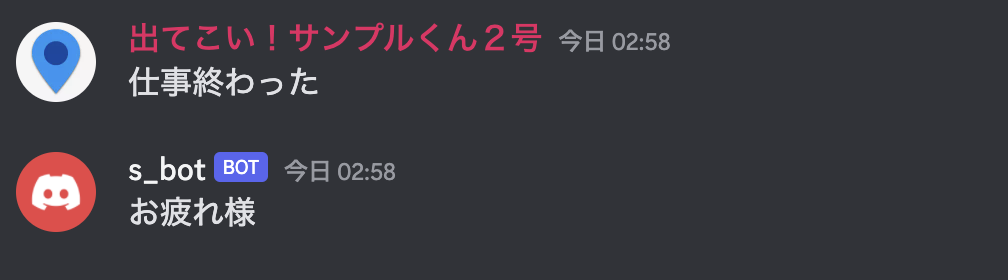
\includegraphics[width=12cm]{./image/03-Tech/chap1/bot.png}
  \caption{動作例}
\end{figure}
\section{まとめ}
今回はDiscordのBotの作り方を説明しました。上記の「仕事終わった」や「お疲れ様」に当たる部分を変えたりして自分好みに改良してみて下さい。